%!TEX root = ../../../memoria.tex
\section{Arquitectura del \frameworkPC}\label{cap:arquitectura:section:arquitectura_framework}

\subsection{\packagesAS}

A continuación se describen las funcionalidades de cada uno de los \packagesAS que actualmente existen. La estructura se encuentra en \refFigura{cap:avances:current_architecture}.

\tikzset{
  basic/.style  = {draw, text width=2cm, drop shadow, font=\sffamily, rectangle},
  root/.style   = {basic, rounded corners=2pt, thin, align=center,
                   fill=green!30},
  level 2/.style = {basic, rounded corners=6pt, thin,align=center, fill=green!60,
                   text width=8em},
  level 3/.style = {basic, thin, align=left, fill=pink!60, text width=6.5em}
}
\begin{figure}[H]
	\centering
	
	
	\begin{tikzpicture}[
	  level 1/.style={sibling distance=40mm},
	  edge from parent/.style={->,draw},
	  >=latex]

	% root of the the initial tree, level 1
	\node[root] {\eframeworkAF}
	% The first level, as children of the initial tree
		child {node[level 2] (c1) {\eframeworkCorePCKG}}
		%child {node[level 2] (c2) {\eframeworkHelloWorldPCKG}}
		child {node[level 2] (c3) {\eframeworkAccountsPCKG}}
		%child {node[level 2] (c4) {rtcom-shipping}}
		child {node[level 2] (c5) {\eframeworkPaypalPCKG}};
		%child {node[level 2] (c6) {\eframeworkGoogleanalPCKG}};
	\end{tikzpicture}
	\caption{\architectureCPT actual de la solución.}
	\label{cap:avances:current_architecture}
\end{figure}
	\begin{itemize}
		\item
			\textbf{\eframeworkAF} es un \frameworkPC \ecommerceCOM desarrollado con \meteorNAME, \nodejsNAME, \mongodbNAME, con un enfoque \reactive y \realTimeINT.
		\item
			\textbf{\eframeworkCorePCKG} corresponde al \coreAS de la solución. Contiene todas aquellas \featuresCPT básicas y \templatesAS a una plataforma \ecommerceCOM tales como manejo de \itemsCOM, \sessionsINT, shipping, ordenes de compra, carro de compra.
		\item
			\textbf{\eframeworkAccountsPCKG} es el \moduleAS para el manejo de cuentas.
		\item
			\textbf{\eframeworkCoreThemePCKG}
		\item
			\textbf{\eframeworkBootstrapThemePCKG}
		\item
			\textbf{\eframeworkShippingPCKG}
		\item
			\textbf{\eframeworkPaypalPCKG}
		
		% \item
		% 	\textbf{\eframeworkHelloWorldPCKG} es un \moduleAS para prueba de conceptos.
	\end{itemize}


La arquitectura descrita en la \refSection{cap:arquitectura:section:generic_arquitectura} fue diseñada para facilitar las implementaciones de cada uno de los \packagesAS que se desarrollen en los proyectos de \meteorNAME. En particular para el proyecto que se desarrolla en este informe se utiliza dicha estructura principalmente en el \packagesAS \coreAS de la aplicación.

\subsubsection{\eframeworkCorePCKG}

Como su nombre lo indica, este \packagesAS corresponde al \coreAS del \frameworkPC conteniendo todas aquellas caracteristicas intrínsecas que dan vida a un sitio \ecommerceCOM. 

\subsubsection{\eframeworkCoreThemePCKG}\label{chapter:section:subsection:package_core_theme}

Este \packagesAS es la base del \bootstrap \themeCPT del \frameworkPC de \ecommerceCOM. Este contiene todos los archivos \lessNAME utilizados para el proceso que genera los archivos \lessNAME personalizado para el \frameworkPC. Este \packagesAS puede ser copiado para crear \themeCPT adicinales para el \frameworkPC \ecommerceCOM.

La implementación de este \packagesAS esta soportada sobre \bootstrapPackage permitiendo sencillamente hacer todas aquellas configuraciones que se desean. \bootstrapPackage permite, entre otras cosas, indicar exactamente cuales son las componentes de \bootstrapNAME que se desean utilizar, así como personalizar e importar el \themeCPT.

A modo de ejemplo, se mostrarán a continuación ejemplos de importaciones de \themesCPT en el \frameworkPC. Para esto se utilizará los \themesCPT gratuitos que proporciona \bootswatchNAME. Esta tarea es muy sencilla, y basta con agregar el \refsource{source:less:generic_bootswatch_theme} al final del arhivo generado por \bootstrapPackage llamado \textbf{custom.reaction.import.less}.

% import codigo 
%%!TEX root = ../../../memoria.tex

\medskip
\begin{lstlisting}[caption= Código genérico para importar \themesCPT de ., label=source:less:generic_bootswatch_theme]
	@import "http://bootswatch.com/THEME_NAME/bootswatch.less";
	@import "http://bootswatch.com/THEME_NAME/variables.less";
\end{lstlisting}
\medskip
\begin{lstlisting}[caption= Código genérico para importar \themesCPT desde \bootswatchNAME, label=source:less:generic_bootswatch_theme]
	@import "http://bootswatch.com/THEME-NAME/bootswatch.less";
	@import "http://bootswatch.com/THEME-NAME/variables.less";
\end{lstlisting}

En donde \textbf{THEME-NAME} corresponde a algún \themeCPT de los disponibles en el sitio de \bootswatchNAME. En particular, los \themesCPT \textbf{\themeSandstone}, \textbf{\themeJournal}, \textbf{\themeCyborg} y \textbf{\themeSuperHero} se pueden apreciar en la \refFigura{figure:bootstrap:theme_standstone}, \ref{figure:bootstrap:theme_journal}, \ref{figure:bootstrap:theme_cyborg} y \ref{figure:bootstrap:theme_superhero} respectivamente.


\begin{figure}[H]
	\centering
	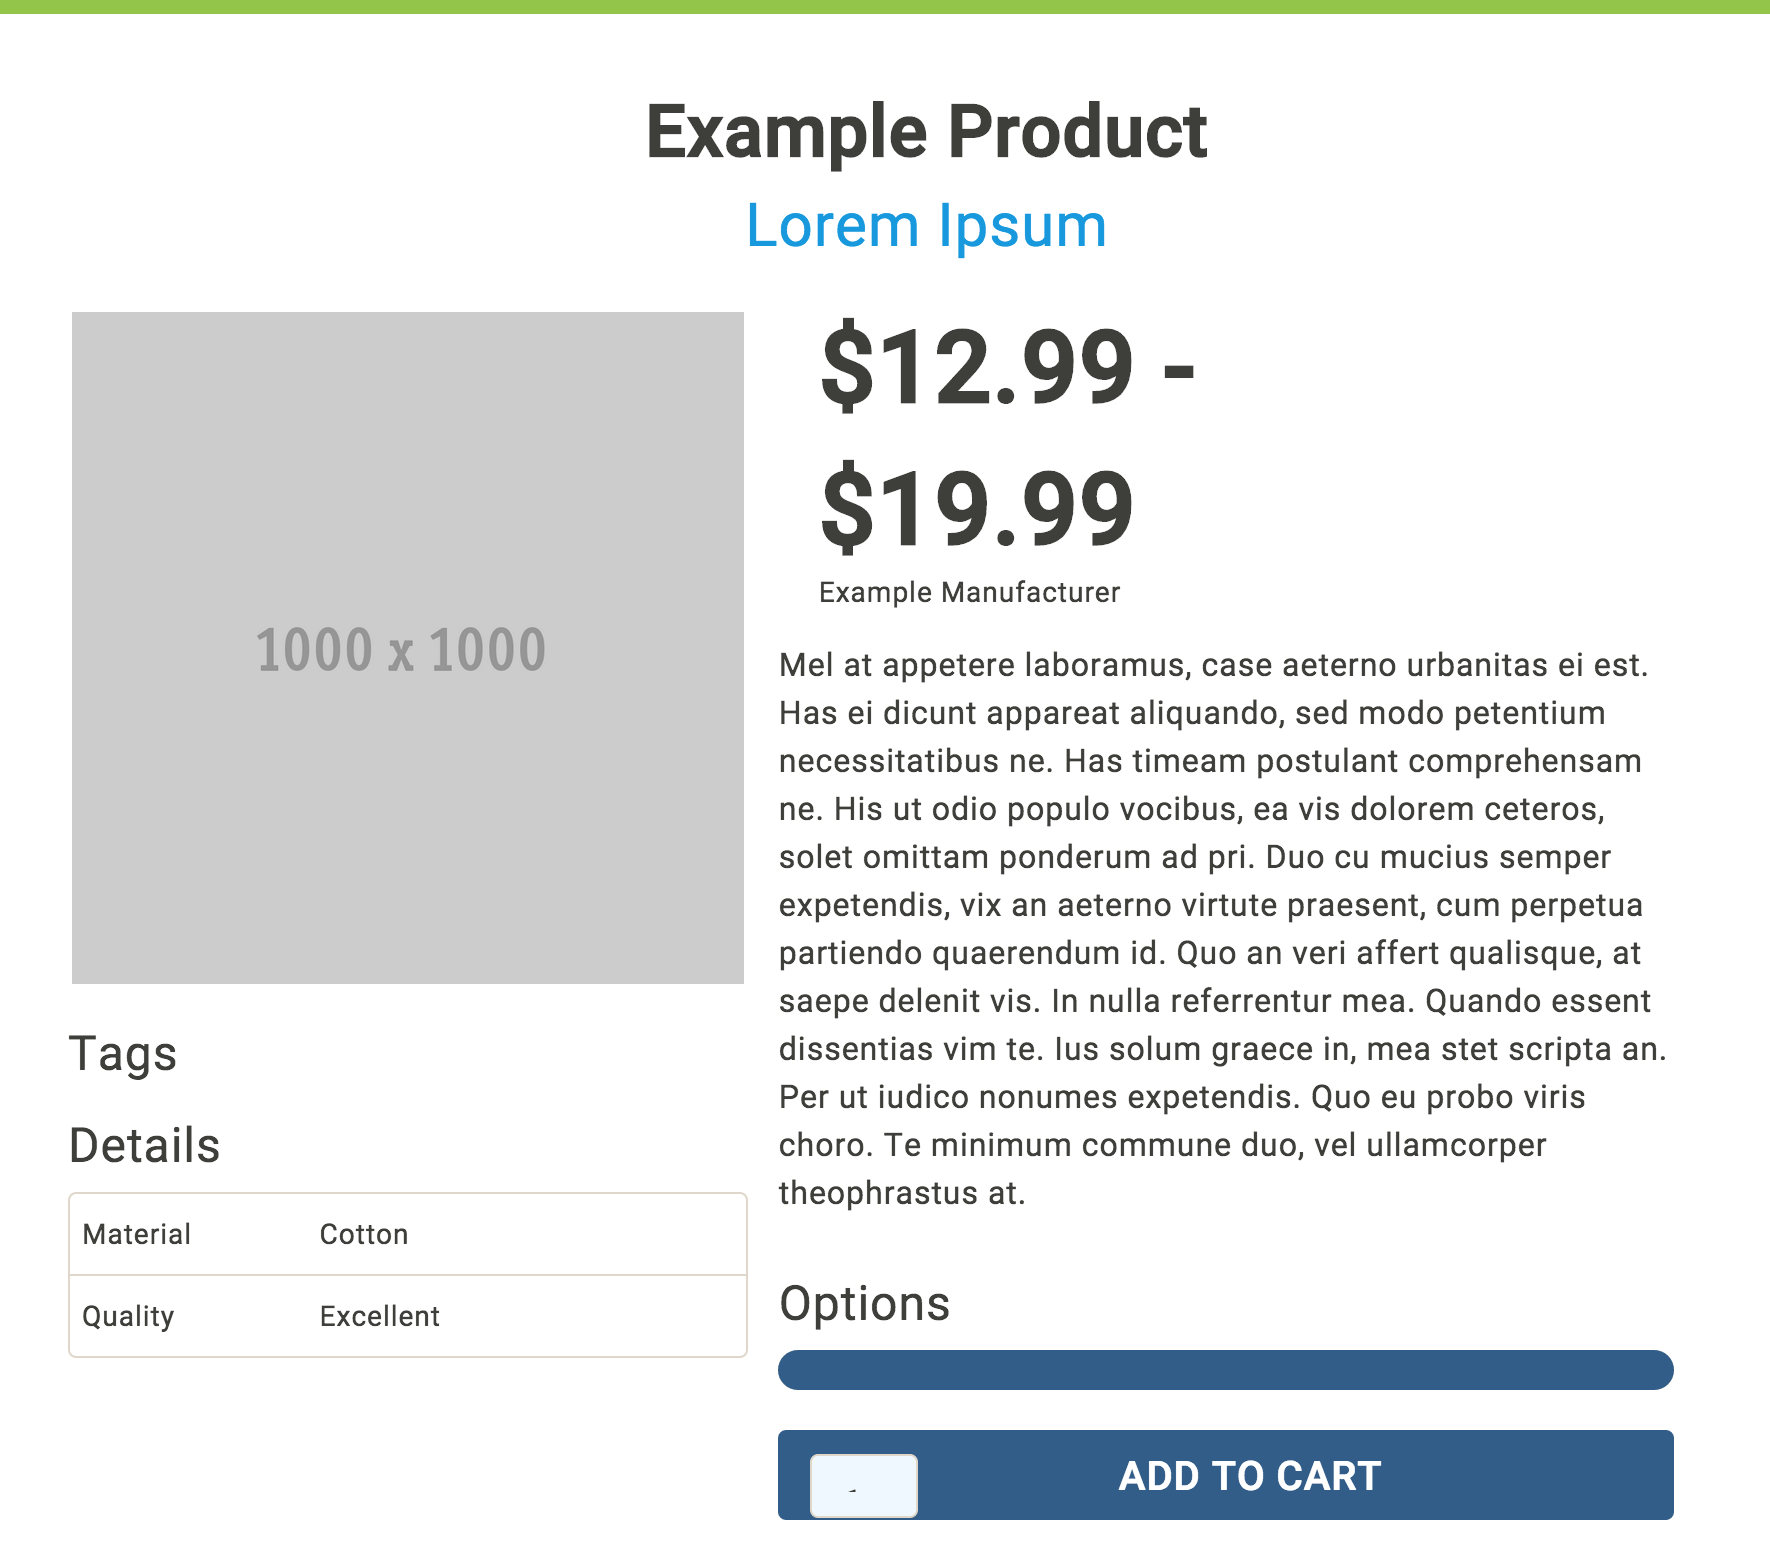
\includegraphics[width=0.6\textwidth]{figuras/bootstrap/bootstrap_theme_sandstone.png}

	\caption{Descripción de un producto utilizando el \themeCPT \textbf{\themeSandstone} del sitio \bootswatchNAME.}
	\label{figure:bootstrap:theme_standstone}
\end{figure}

\begin{figure}[H]
	\centering
	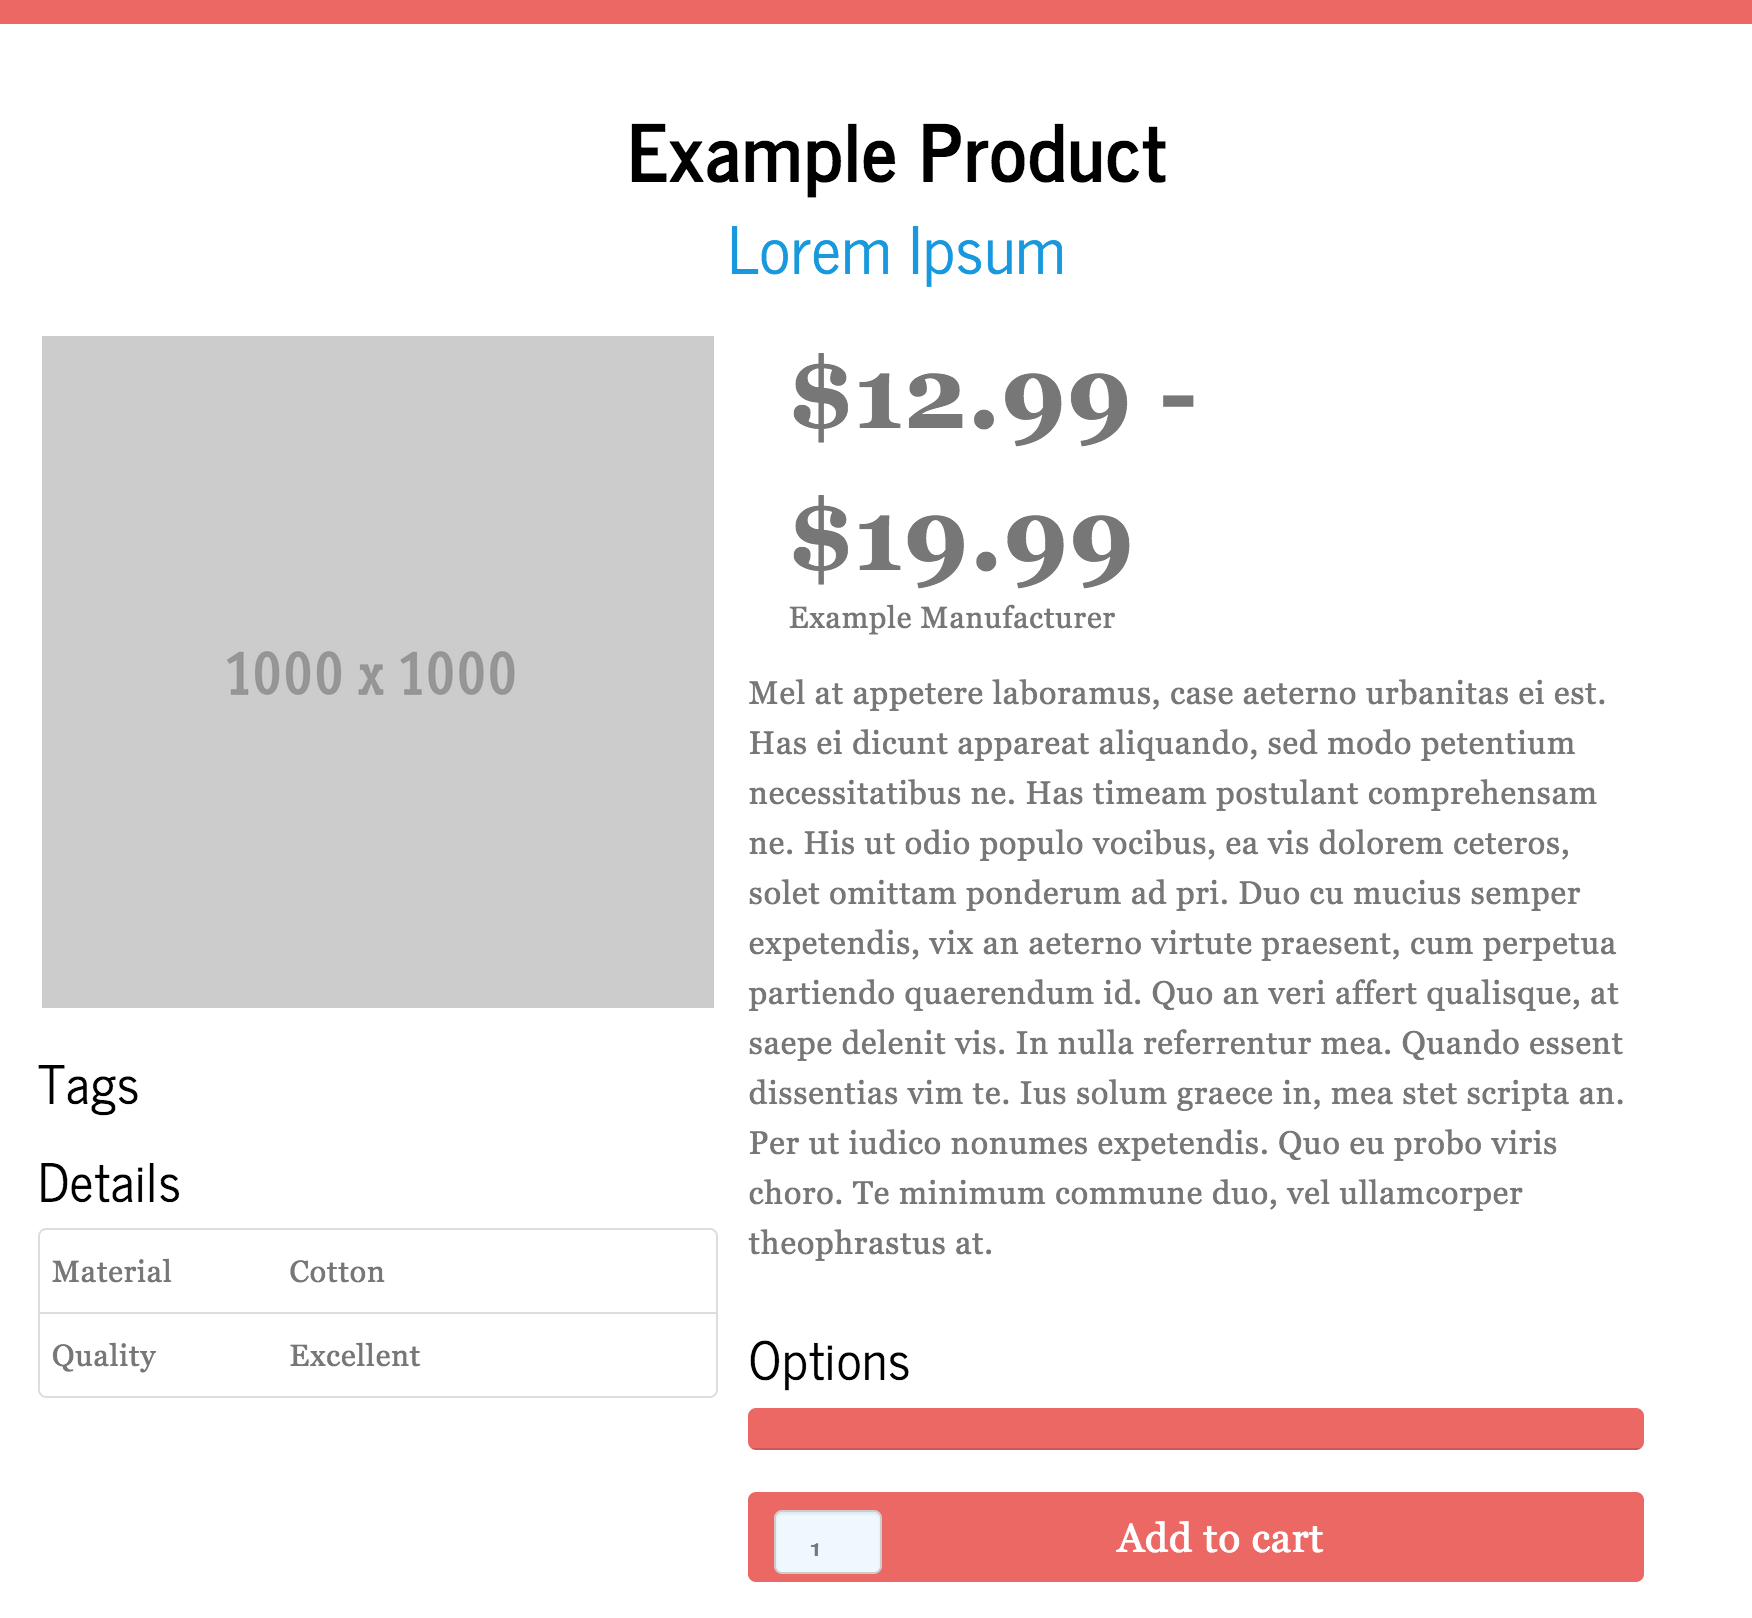
\includegraphics[width=0.6\textwidth]{figuras/bootstrap/bootstrap_theme_journal.png}

	\caption{Descripción de un producto utilizando el \themeCPT \textbf{\themeJournal} del sitio \bootswatchNAME.}
	\label{figure:bootstrap:theme_journal}
\end{figure}

\begin{figure}[H]
	\centering
	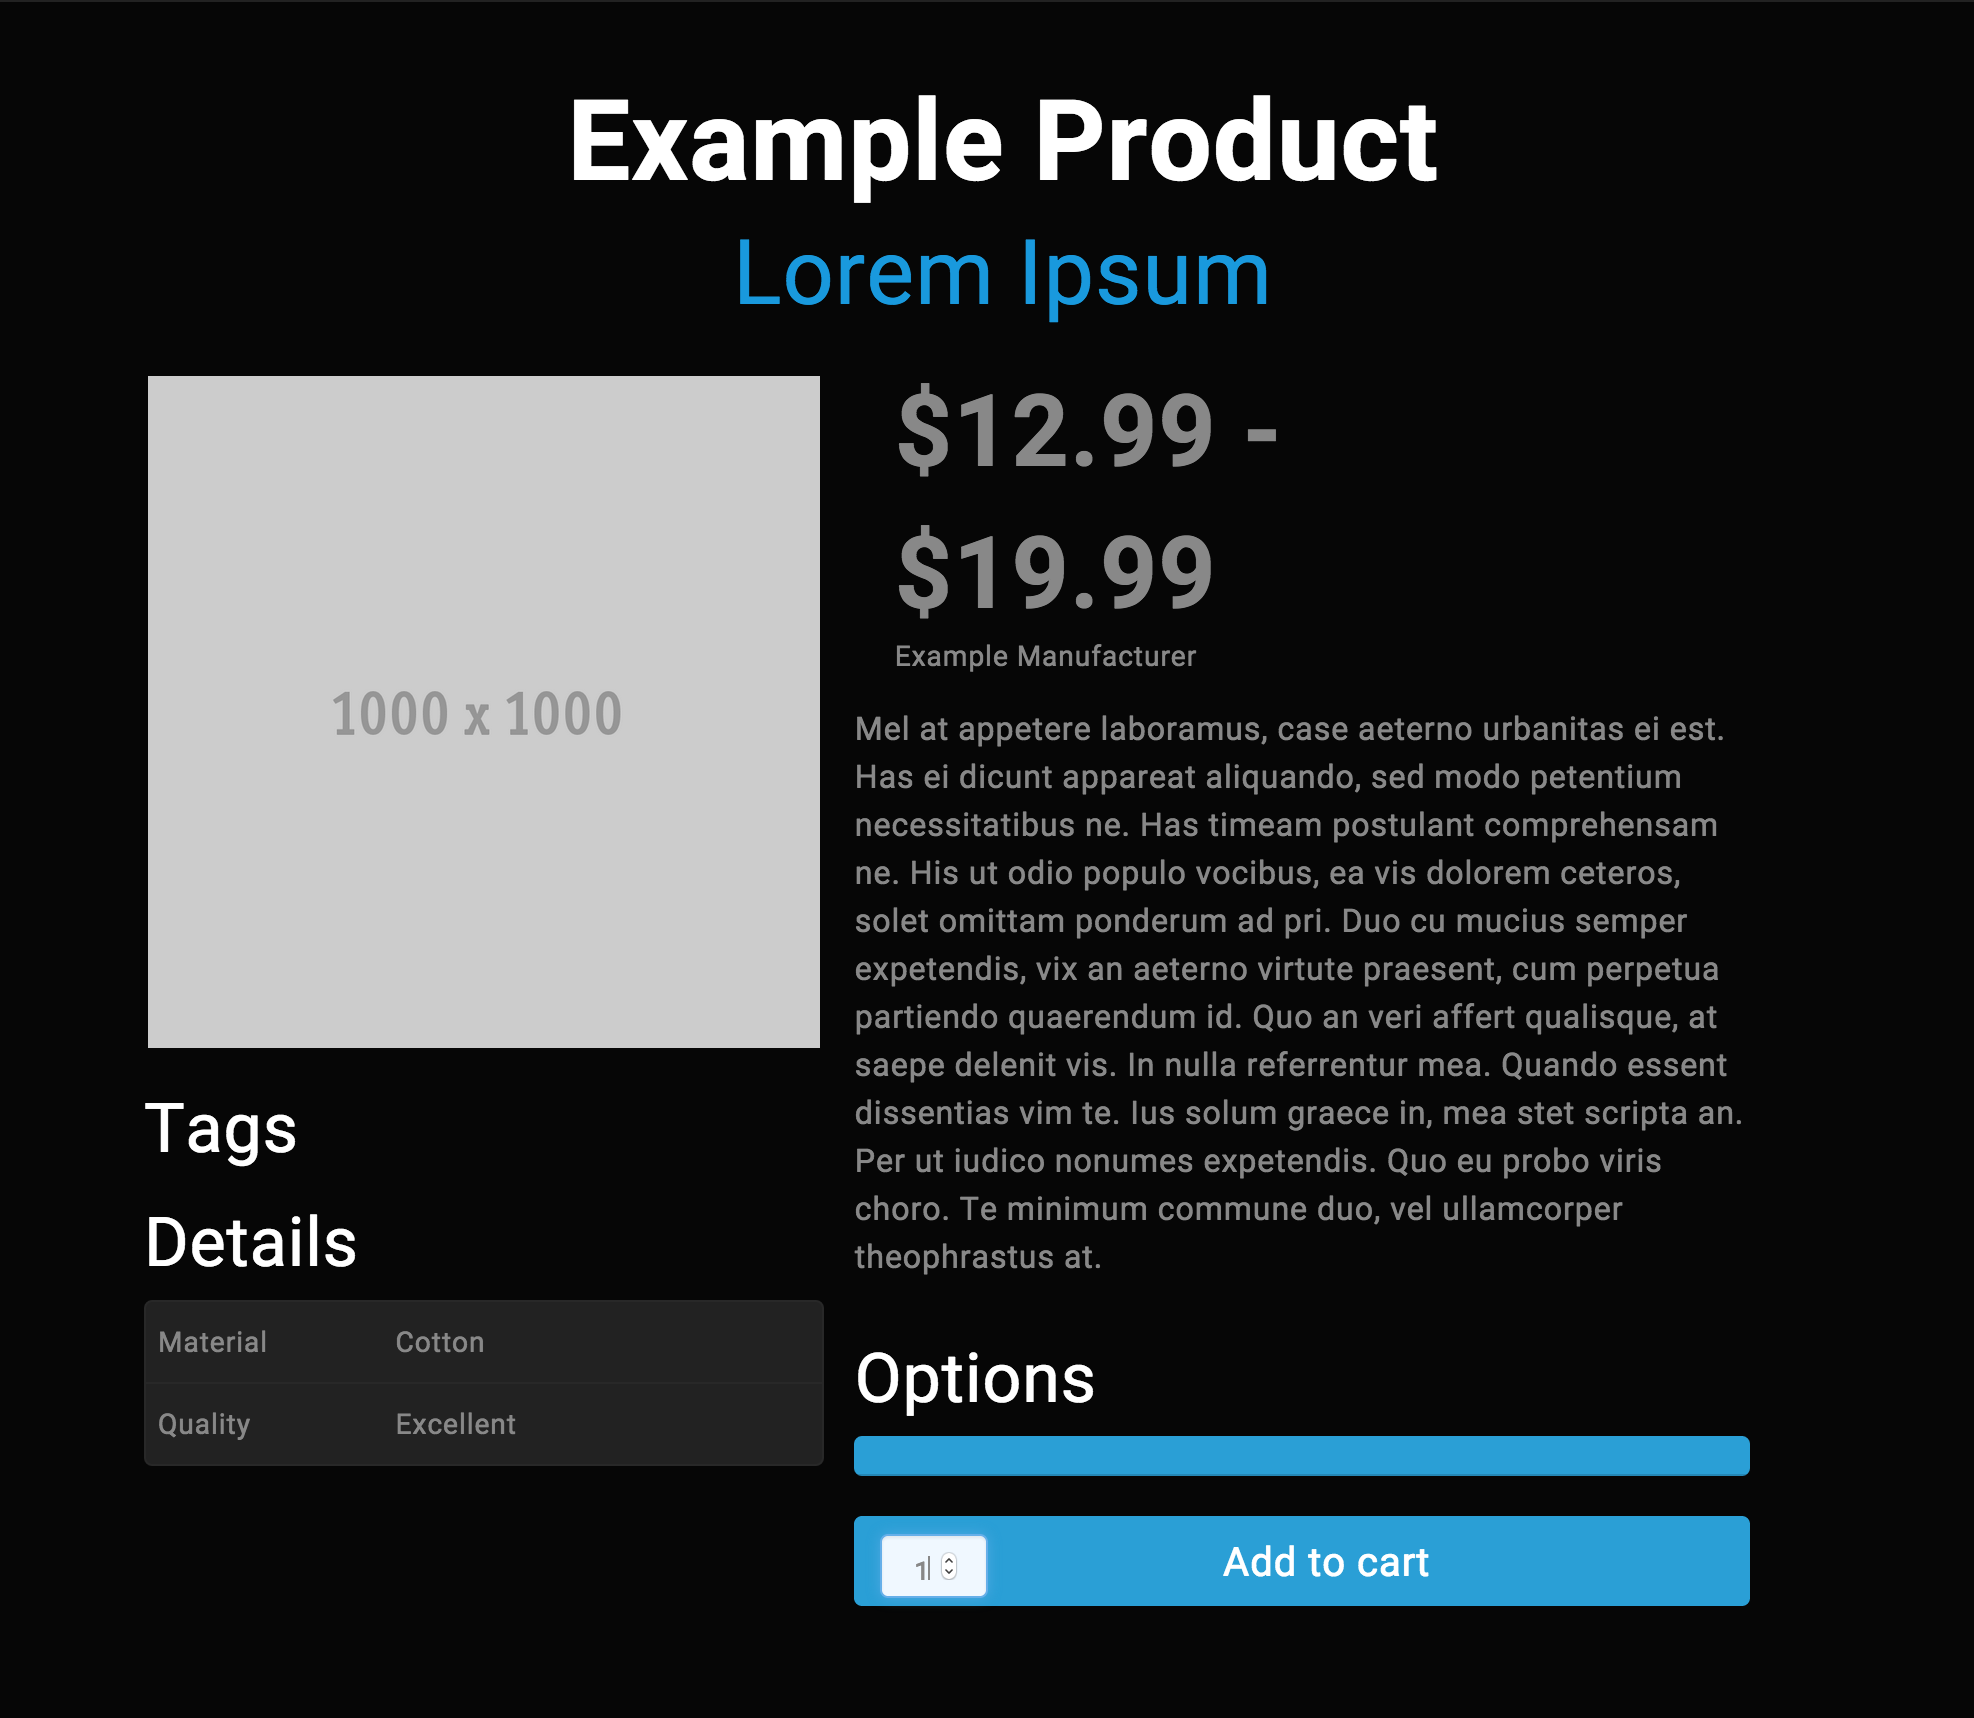
\includegraphics[width=0.6\textwidth]{figuras/bootstrap/bootstrap_theme_cyborg.png}

	\caption{Descripción de un producto utilizando el \themeCPT \textbf{\themeCyborg} del sitio \bootswatchNAME.}
	\label{figure:bootstrap:theme_cyborg}
\end{figure}


\begin{figure}[H]
	\centering
	\includegraphics[width=0.6\textwidth]{figuras/bootstrap/bootstrap_theme_superhero.png}

	\caption{Descripción de un producto utilizando el \themeCPT \textbf{\themeSuperHero} del sitio \bootswatchNAME.}
	\label{figure:bootstrap:theme_superhero}
\end{figure}

\subsubsection{\eframeworkCorePCKG}

% Sección que habla sobre los workflows en el framwork
%!TEX root = ../../../memoria.tex

\subsection{\workflowsCPT}

%TODO
% Introduccion de workflows

Existen una serie de pasos que se pueden experimentar al visitar un sitio \ecommerceCOM, entre los cuales podemos destacar:

	\begin{itemize}
		\item
			\textbf{Shopping Experience}.
		\item
			\textbf{Order Capture} 
		\item
			\textbf{Order Fullfillment} 
		\item
			\textbf{Order processing}
		\item
			\textbf{Shipping} 
		\item
			\textbf{Customer Files} 
		\item
			\textbf{Paymanat Sistems} 
		\item
			\textbf{Customer Service} 
		\item
			\textbf{Accounting} 
		\item
			\textbf{Returning} 
	\end{itemize}


Cada uno de los pasos dentro de un \workflowsCPT puede ser considerado como un estado el cual cambiará dependiendo de los eventos que esten involucrados. Por lo tanto cada uno de estos \workflowsCPT puede ser modelado utilizando una máquina de estados finitos.
Para el caso particular del \frameworkPC para \ecommerceCOM, 4 han sido los \workflowsCPT que han sido implementados utilizando la librería \javaScriptNAME \finiteStateMachine.

\begin{figure}[H]
	\centering
	\includegraphics[width=1.1\textwidth]{figuras/cart_state_machine.jpg}

	\caption{Máquina de estado de carro de compras.}
	\label{figure:cart_state_machine}
\end{figure}


\begin{figure}[H]
	\centering
	\includegraphics[width=0.8\textwidth]{figuras/order_state_machine.jpg}

	\caption{Máquina de estado del estado de una orden.}
	\label{figure:order_state_machine}
\end{figure}

